\documentclass{beamer}
\usepackage{listings}
\lstset{
%language=C,
frame=single, 
breaklines=true,
columns=fullflexible
}
\usepackage{blkarray}
\usepackage{subcaption}
\usepackage{url}
\usepackage{tikz}
\usepackage{tkz-euclide} % loads  TikZ and tkz-base
%\usetkzobj{all}
\usetikzlibrary{calc,math}
\usepackage{float}
\newcommand\norm[1]{\left\lVert#1\right\rVert}
\renewcommand{\vec}[1]{\mathbf{#1}}
\usepackage[export]{adjustbox}
\usepackage[utf8]{inputenc}
\usepackage{amsmath}
\usepackage{tikz}
\usetikzlibrary{automata, positioning}
\usetheme{Boadilla}
\providecommand{\pr}[1]{\ensuremath{\Pr\left(#1\right)}}
\providecommand{\brak}[1]{\ensuremath{\left(#1\right)}}
\providecommand{\sbrak}[1]{\ensuremath{{}\left[#1\right]}}
\DeclareMathOperator*{\max}{max}
\title{Application of Hidden Markov Models in Stock Trading (2020)}
\author{Vaishnavi W}
\institute{IITH AI}
\date{AI20BTECH11025}
\begin{document}

\begin{frame}
\titlepage
\end{frame}
\begin{frame}
\frametitle{Hidden Markov Models}
\begin{columns}
\begin{column}{0.5\textwidth}
\begin{figure}
\begin{flushleft}
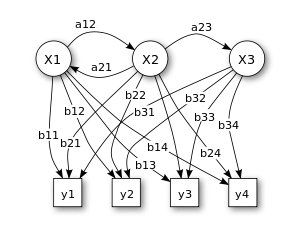
\includegraphics[width=\columnwidth]{hmm3.png}
\end{flushleft}
\end{figure}
\end{column}
\begin{column}{0.5\textwidth}
Probabilistic parameters of a hidden Markov model 
\begin{enumerate}
    \item X — states 
    \item y — possible observations 
    \item $a_{ij}$ — state transition probabilities 
    \item $b_{ij}$ — output probabilities 
\end{enumerate}

\end{column}
\end{columns}

\end{frame}
\begin{frame}{Hidden Markov Models}
 \begin{figure}[H]
\centering
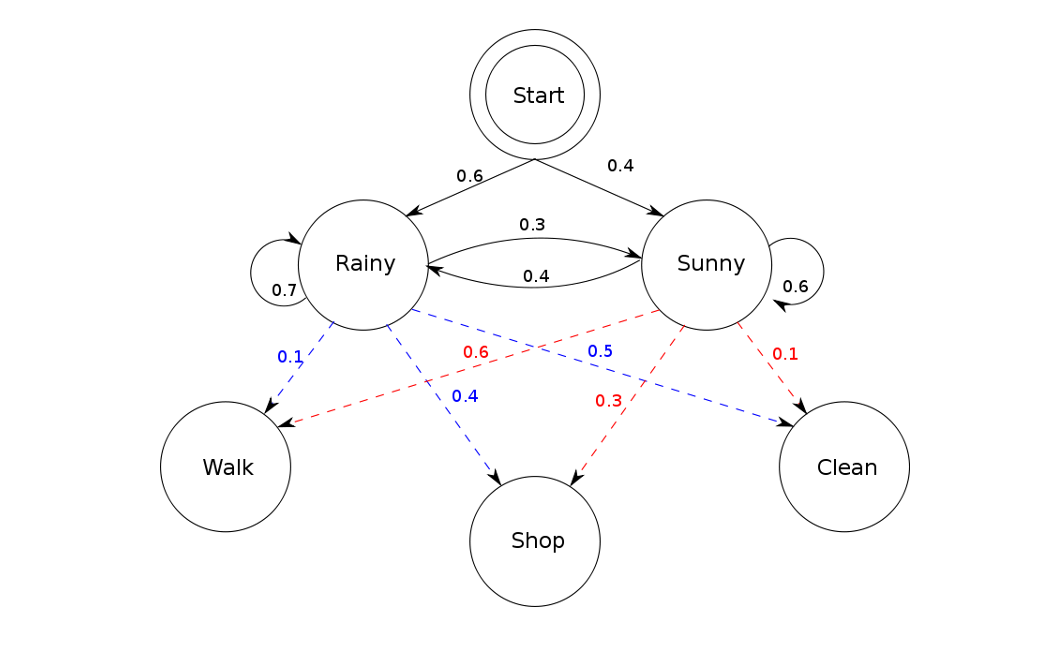
\includegraphics[width=\columnwidth]{hmm2.png}
\caption{HMM example}
\label{fig1}
\end{figure}
\end{frame}


\begin{frame}
\frametitle{Components of HMM}
\begin{enumerate}
    \item Set of N hidden states represented by Q = \{$q_1,q_2,\dots,q_N$\}
    \item Transition Probability Matrix: Probability of moving from one state to another. $a_{ij}$ - probability of moving from state i to state j.
\begin{align}
\label{eq:A}
A=\begin{blockarray}{ccc}
&R & S  \\
\begin{block}{c[cc]}
  R & 0.7 & 0.3  \\
  S & 0.4 & 0.6  \\
\end{block}
\end{blockarray}
\label{eq:B}
\end{align}
 \item Observation Likelihood: Also called emission probabilities, the probability of an 
observation being generated from a state i.

$b_i\brak{o_t}$ - probability of state \brak{i} generating observation $o_t$
    
 Let B be the set of all emission probabilities.
\end{enumerate}
\end{frame}

\begin{frame}
\frametitle{Components of HMM contd.}
\begin{enumerate}
\setcounter{enumi}{3}
 \item Initial Probability Distribution: The probability that the Markov chain starts at a state (i)
\begin{align}
\label{eq:pi}
\pi=\begin{blockarray}{cc}
\begin{block}{[cc]}
  0.6&0.4
\end{block}
\end{blockarray}
\label{eq:C}
\end{align}
    \item Sequence of T observations: O = \{$o_1,o_2,\dots,o_T$\}
    
    For example: W, W, C, S, C
\end{enumerate}
HMM model is represented as $\lambda = \brak{ A, B, \pi}$
\end{frame}

\begin{frame}{Assumptions of HMM}
\begin{enumerate}
    \item The probability of being in a particular state depends only on the previous state  i.e 
    \begin{align}
    \pr{q_{t+1}|q_{t},q_{t-1},\dots,q_1}=\pr{q_{t+1}|q_{t}}
    \end{align}
     \item The probability of the output observation depends only on the state that produced the observation and not on any other states or any other observations. 
     \begin{align}
    \pr{o_{t}|q_{t},q_{t-1},\dots,q_1,o_{t-1},\dots,o_1}=\pr{o_{t}|q_{t}}
    \end{align}
\end{enumerate}
\end{frame}
\begin{frame}{Three Fundamental Problems of HMM}
\begin{enumerate}
    \item \textbf{Evaluation Problem:} Given an HMM $\lambda = \brak{ A, B, \pi}$ and an observation sequence $O =$ \{$o_1,o_2,\dots,o_T$\}, calculate the probability that the observed sequence was produced by the model. It is about determining the likelihood of the observation sequence - \pr{O|\lambda}. This is solved using \textbf{Forward or Backward algorithm}
    \item \textbf{Decoding Problem:} Given an HMM $\lambda$ and an observation sequence $O$, find the optimal hidden state sequence $Q= q_1,q_2,\dots,q_t$ that can best explain the observations. This is solved using \textbf{Viterbi algorithm}
    \item \textbf{Learning Problem:} Given a sequence of observations $O$ and the number of hidden and visible states, find the HMM parameters $\lambda$ that best fit the training data.  
\end{enumerate}
\end{frame}

\begin{frame}{Training HMM}
    HMMs are trained using Expectation Maximization Algorithm. EM algorithm is an iterative method to find maximum likelihood of parameters in statistical models, where the model depends on unobserved variables.
    \begin{enumerate}
        \item Set $\lambda =(A,B,\pi )$ with random initial conditions.
        \item E-step : Updates the parameters and computes the expected value of the log-likelihood using the current estimate for the parameters
        \item M-step : Computes parameters maximizing the expected log-likelihood found on the E step
    \end{enumerate}
    Steps 2 and 3 are iterated till the values converge.
\end{frame}
\begin{frame}{Why HMM for Stock Market Prediction?}
    HMMs are based on a set of unobserved underlying states amongst which transitions can occur and each state is associated with set of possible observations. Stock markets can be seen in a similar way. The underlying states, which determine the behavior of the stock value, are usually invisible to the investor. The transitions between these underlying states are based on company policy, decisions and economic conditions etc. The visible effect which reflects these is the value of the stock.
    
    Clearly, the HMM conforms well to this real life scenario.
\end{frame}
\begin{frame}{Data Description for Stock Market Prediction}
    The data considered for the study includes the 5 selected stock indices: S&P 500, DowJones, NIFTY 50, KOSPI and New York Stock Exchange (NYSE).The data is been collected through the stock Exchanges for about 5 years 2014-2019. The data collected for the study approximates to 1387 data points. Around 6 attributes are been captured. The daily stock indices data includes High Price, Low Price, Close Price, Open Close, Volume and Adjusted Volume. 
    
    Data Analysis : The closing price of the stock indices is given as the input and the market behaviour is estimated based on the emission and transition probabilities.
\end{frame}

\begin{frame}{AIC and BIC}
     The criteria used to select the best model are Akaike information criterion (AIC) and Bayesian information criterion (BIC). They are penalized loglikelihood criterion. They are given as,
    \begin{align}
        AIC = -2 LL + 2p\\
        BIC = -2 LL + plog(n)
    \end{align}
    LL - loglikelihood of the model 
    
    p - number of independent parameters in the model
    
    n - number of data points in the training data set
    
    The model with the lowest AIC and BIC is selected.
    
    AIC penalizes complex models less, meaning that it may put more emphasis on model performance while BIC penalizes the model more for its complexity.
    
    The number of states of the HMM are limited to five to keep the model simple and feasible with cyclical economic stages.
\end{frame}
\begin{frame}{NIFTY 50}
\begin{figure}[H]
\centering
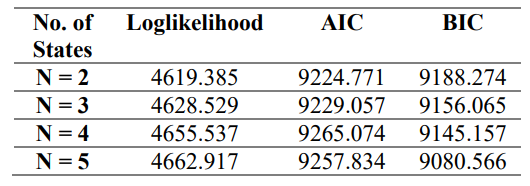
\includegraphics[width=\columnwidth]{hmm6.png}
\caption{HMM Models for NIFTY 50}
\label{fig3}
\end{figure}

\end{frame}
\begin{frame}{2 Hidden States}
\begin{figure}[H]
\centering
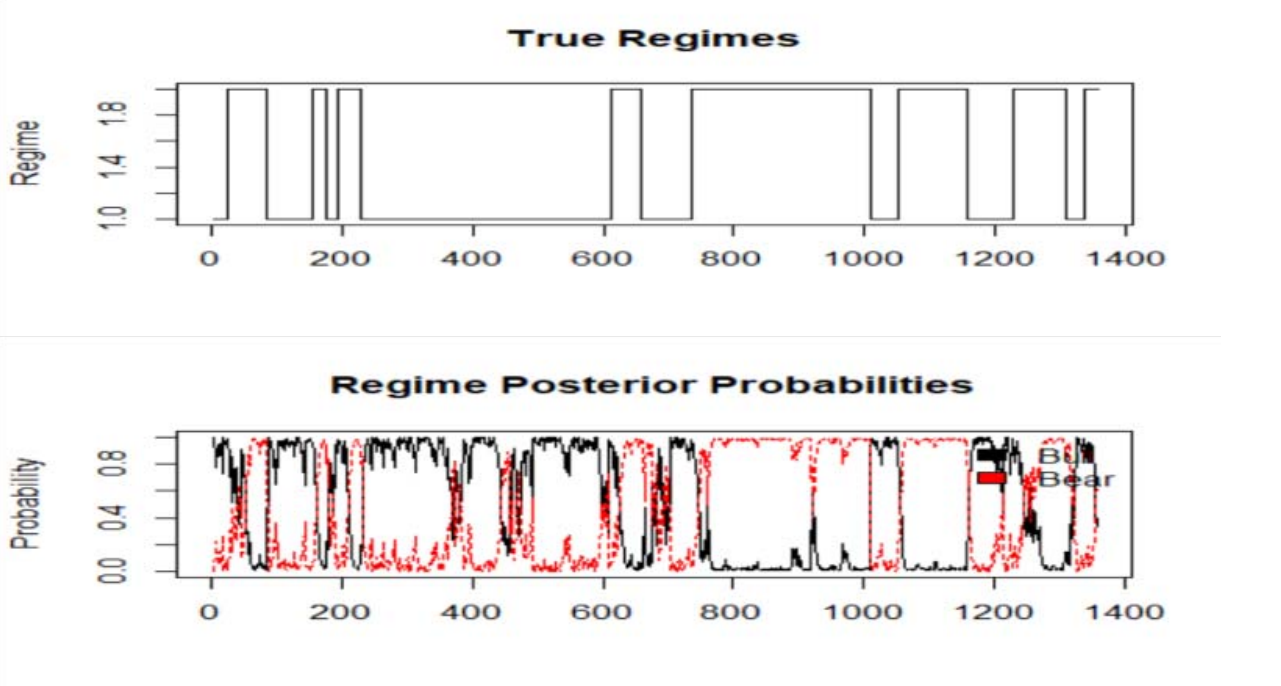
\includegraphics[width=\columnwidth]{501.png}
\caption{Graph showing regime probabilities and the hidden states when number of states is 2}
\label{fig4}
\end{figure}    
\end{frame}
\begin{frame}{3 Hidden States}
\begin{figure}[H]
\centering
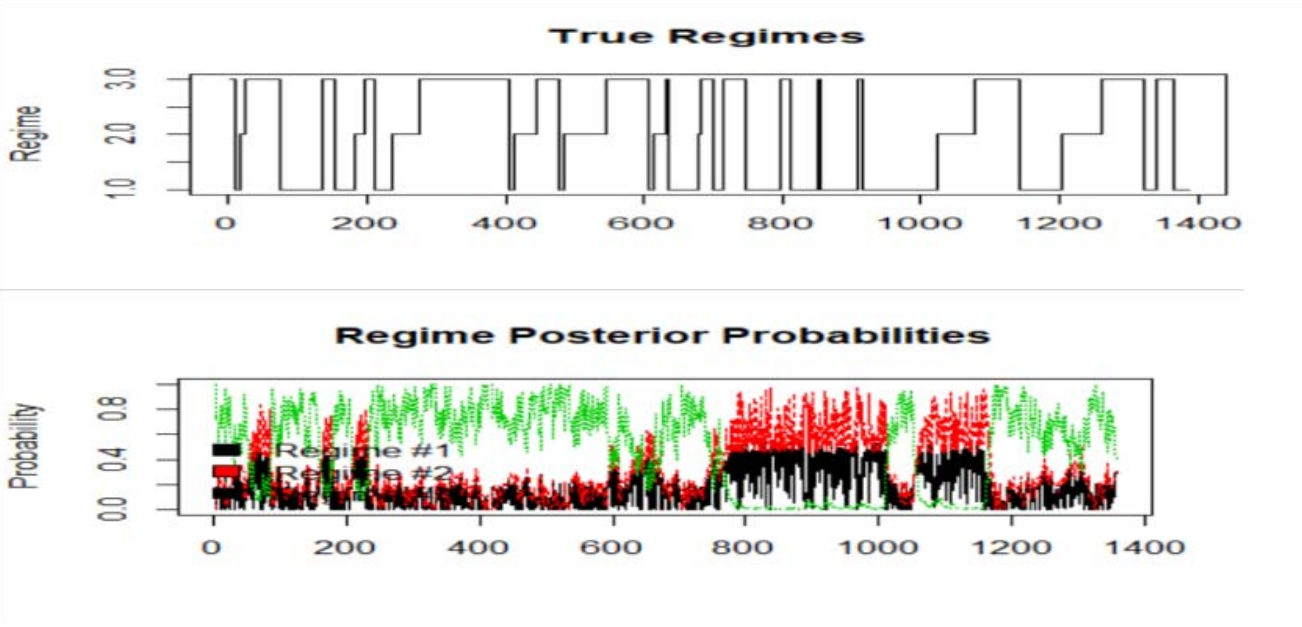
\includegraphics[width=\columnwidth]{502.png}
\caption{Graph showing regime probabilities and the hidden states when number of states is 3}
\label{fig5}
\end{figure}    
\end{frame}
\begin{frame}{4 Hidden States}
\begin{figure}[H]
\centering
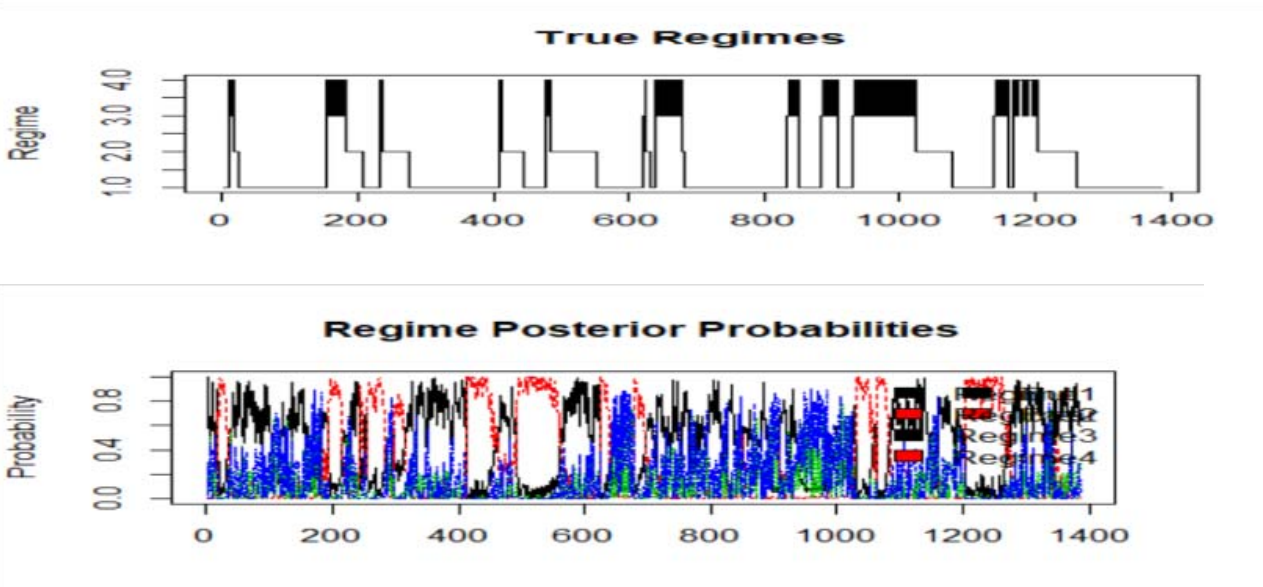
\includegraphics[width=\columnwidth]{503.png}
\caption{Graph showing regime probabilities and the hidden states when number of states is 4}
\label{fig6}
\end{figure}    
\end{frame}
\begin{frame}{5 Hidden States}
\begin{figure}[H]
\centering
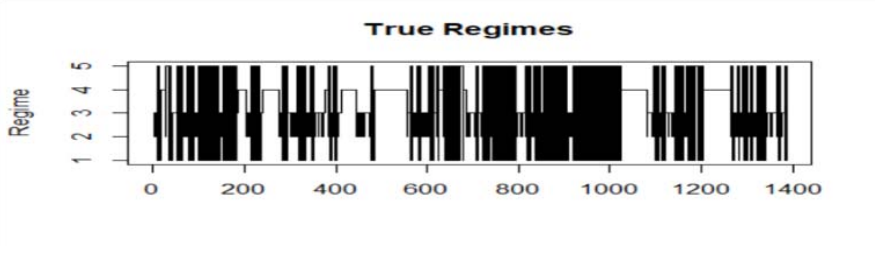
\includegraphics[width=\columnwidth]{hmm7.png}
\end{figure}
\begin{figure}[H]
\centering
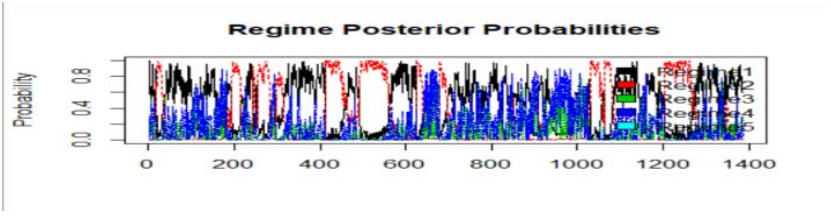
\includegraphics[width=\columnwidth]{hmm8.png}
\caption{Graph showing regime probabilities and the hidden states when number of states is 5}
\label{fig7}
\end{figure}    
\end{frame}
\begin{frame}{Conclusion :}
    Similarly, HMM models were trained with the data of other stock indices. After considering the AIC and BIC values of all the models, it was found models with two hidden states have lower AIC and BIC values i.e all the markets show two hidden states. Hence, for the investors to decide on their investment plan, one has to look whether the market is moving uptrend or downtrend specifying bullish and bearish market. 

Also, by applying further ML techniques the closing prices can be predicted.

\end{frame}
\end{document}